\chapter{Implementación y análisis de algoritmos}

En este apartado se realizará un análisis detallado sobre cómo funciona cada uno de los algoritmos seleccionados para el estudio desde un punto de vista teórico. Se explicarán las técnicas que utiliza cada uno para llegar a la solución óptima y cómo se asemejan dichas técnicas al comportamiento humano, para de ese modo poder considerarse un algoritmo socioinspirado. Además, se arrojarán detalles destacados de la implementación de cada uno en particular, si dicha implementación así lo requiriese.

Los algoritmos se analizarán en orden cronológico, siendo el más antiguo de todos Imperialist Competitive Algorithm (2007) \cite{ica-conference} y el más reciente Ideology Algorithm (2016) \cite{ia-article}.

\section{Detalles generales sobre la implementación}

En primer lugar, antes de comenzar con la explicación de los algoritmos, conviene dar una visión general acerca de la implementación en este estudio, cómo se ha llevado a cabo y con qué herramientas.

Los algoritmos se han implementado utilizando el lenguaje de programación \textbf{Python} en su versión 3.6 \cite{python-3.6-doc}, elección personal del alumno, dada su facilidad para trabajar con vectores y matrices utilizando librerías como \textbf{Numpy} \cite{numpy-doc}, además de otras de representación gráfica como \textbf{Matplotlib} \cite{matplotlib-doc}. Poder operar de forma sencilla con múltiples matrices que habitualmente constituirán la población de soluciones de cada problema resultó un detalle determinante para tomar la decisión.

Encontrar el código fuente de los algoritmos mencionados resulta una ardua tarea, ya que la mayoría de los autores no liberan su código en ninguna plataforma. En algunas ocasiones es posible encontrar versiones en el lenguaje de programación \textbf{MATLAB}, uno de los lenguajes más utilizados en el ámbito científico y de investigación por su capacidad de cómputo y de operar con fórmulas matemáticas de gran dimensión. Sin embargo, MATLAB es un software privativo y de pago, y el alumno ha querido liberar su proyecto desde el primer momento, por lo que se rechazó la idea de implementarlos en este lenguaje. Sin embargo, sí que se ha utilizado como referencia para algún algoritmo una versión de MATLAB sobre la que basar la implementación en Python.

En relación a lo comentado en el párrafo anterior, el proyecto ha estado libre y alojado en la plataforma \textbf{GitHub} \cite{repositorio-tfg} desde que se comenzó la implementación, para que cualquier usuario interesado pudiese no sólo acceder a él sino también comprobar cómo está hecho, y en un futuro incluso realizar los cambios pertinentes que considerase, cumpliendo así el paradigma del software libre.

\section{Imperialist Competitive Algorithm (ICA)}

El primer algoritmo a analizar, \textbf{Imperialist Competitive Algorithm} o, según sus siglas, \textbf{ICA}, fue presentado por primera vez en 2007 por Atashpaz-Gargari y Lucas \cite{ica-conference}. Se trata de un algoritmo que podría ser agrupado en la subcategoría de socioinspirados basados en conquistas y colonialismo, como lo han hecho Kumar et al. \cite{socio-evolution-algorithm}.

La implementación del ICA en Python no pudo ser encontrada en internet, sin embargo sí que se encontró el código fuente en MATLAB, subido por el propio autor del \textit{paper} \cite{ica-matlab}. Este código se ha usado como referencia para implementarlo de forma similar en Python, ya que algunos detalles varían con respecto a la literatura.

Este algoritmo parte de la idea de un mundo completamente colonialista, plagado de países que luchan por alzarse vencedores y conquistadores. En esta guerra constante, los países con más poder se volverían los líderes, y podrían contar con numerosas colonias a su servicio. Por otra parte, aquellos países que no pueden vencer a los demás se verían relegados a ocupar un puesto de colonia para siempre.

Durante la guerra también se puede producir una revolución o alzamiento de una de las colonias contra su propio imperio. Si esta colonia resulta ser más poderosa que el actual líder, dicha posición pasa a ser suya. También puede darse el caso totalmente opuesto; si una colonia resulta realmente débil, un imperio colindante puede absorberla y hacerse más fuerte gracias a ella. Y por supuesto, un imperio puede ser colonizado al completo por otro, haciéndose así cargo de sus colonias restantes y del propio país imperial.

En palabras de los propios autores del algoritmo, <<la competición imperialista con suerte convergerá a un estado en el que sólo haya un imperio y todas sus colonias se hallen en la misma posición y tengan el mismo coste que el país imperialista>>.

Como se puede observar de esta hoja de ruta del algoritmo, la relación con la sociedad es evidente, aunque recuerde más a épocas pasadas que a la actualidad. Este es el funcionamiento del algoritmo a grandes rasgos, pero a continuación se detallarán las características más llamativas del mismo. Previamente se muestra un pseudocódigo del algoritmo, para ayudar a comprender cada paso del mismo antes de la explicación detallada.

\begin{algorithm}
	\caption{Imperialist Competitive Algorithm}
	\begin{algorithmic}[1]
		\State $imperios \gets \textit{inicializarImperios()}$
		\While{\textbf{not} \textit{criterioParada}}
		\For{\textbf{each} \textit{colonia}}
		\State $colonia \gets colonia + (imperialista - colonia + rand())$
		\If{$peso(colonia) < peso(imperialista)$}
		\State $imperialista \gets colonia$
		\EndIf
		\EndFor
		\State $imperios \gets competicionImperial()$
		\If{\textbf{any} \textit{imperio} \textbf{is empty}}
		\State $imperios \gets eliminarImperio(imperio)$
		\EndIf
		\EndWhile
		\State{\textbf{return} \textit{min(peso(imperialistas))}}
	\end{algorithmic}
\end{algorithm}

Se puede comenzar este análisis en base a los distintos componentes del algoritmo, relacionándolos con la descripción anterior y comprobando por qué se trata de técnicas socioinspiradas.

En primer lugar conviene hablar acerca de la población. Si bien habitualmente en estos algoritmos socioinspirados la población suele estar constituida de individuos, siendo esta una agrupación de los mismos, en el caso del algoritmo ICA no es así. En este algoritmo se realiza un símil con una sociedad global donde cada una de las soluciones que compone la población es como un país, o en este caso como una colonia. Por tanto, la figura del ser humano como persona individual no aparece en esta propuesta.

Una vez que se han instanciado las primeras soluciones o colonias que ocuparán la población inicial, hay que seleccionar aquellas que sean más poderosas para considerarlas <<imperialistas>>, es decir, serán los líderes de cada uno de los imperios en los que se divida el problema. Por supuesto, tanto el número de colonias como el número de imperios iniciales son definidos en los parámetros del algoritmo y pueden variar si así se desea.

A lo largo de todo este algoritmo se entenderá que un país es más poderoso que otro si \textbf{su evaluación para la función objetivo es menor}, dado que se trata de problemas de optimización buscando el menor valor posible. La asignación de los imperios se hace con respecto a las colonias iniciales con un menor valor para dicha función.

Con los imperios constituidos y las colonias distribuidas se comienza a desarrollar el bucle principal del algoritmo, que finalizará cuando se cumpla el criterio de parada. La implementación de este algoritmo originalmente paraba tras un número de <<décadas>> (iteraciones del bucle principal), pero a fin de integrarlo con el resto de algoritmos del estudio se añadió la posibilidad de definir un criterio de parada por número de evaluaciones de la función objetivo.

En cada iteración de dicho bucle cada colonia realiza un desplazamiento hacia su imperialista. El desplazamiento tiene un componente de aleatoriedad que permite que no converjan todas las soluciones en el primer imperialista nada más comenzar las iteraciones. A continuación se puede observar una representación gráfica de dicho movimiento.

\begin{figure}[h]
	\centering
	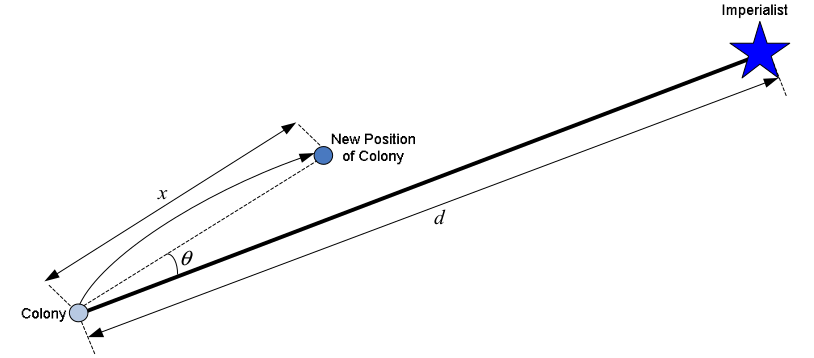
\includegraphics[scale=0.4]{imagenes/ica-desplazamiento.png}
	\caption{Desplazamiento de una colonia hacia su imperialista, con un componente de aleatoriedad \cite{ica-conference}.}
	\label{ica-desplazamiento}
\end{figure}

El movimiento producido $x$ queda definido por la siguiente fórmula

\begin{equation}\label{ica-eq-desplazamiento1}
x \sim U(0, \beta \times d)
\end{equation}

en la cual $d$ es la distancia entre la colonia y el imperialista y $\beta$ representa el llamado <<coeficiente de asimilación>>. Es decir, se trata de un desplazamiento hacia el imperialista donde la distancia recorrida está definida por un valor uniforme aleatorio entre 0 y la máxima distancia.

Además, el ángulo $\theta$ que aparece en la figura, que desvía a la colonia de su dirección, viene calculado de la siguiente forma

\begin{equation}\label{ica-eq-desplazamiento2}
	\theta \sim U(-\gamma, \gamma)
\end{equation}

donde $\gamma$ es el parámetro que ajusta la desviación de la dirección, y que es llamado por los autores <<coeficiente del ángulo de asimilación>>.

Los cambios producidos mediante estos operadores mencionados ayudan a diversificar las posiciones de las colonias y a que no se agrupen automáticamente en torno a la mejor solución del imperio. Esto permite al algoritmo explorar el espacio de búsqueda adecuadamente y no caer en posibles óptimos locales con facilidad en las primeras iteraciones, lo que limitaría mucho el proceso evolutivo. Si la nueva posición hacia la que se mueve una colonia resulta ser mejor que la del actual imperialista de dicho imperio, se intercambian los puestos y el resto de colonias intentará moverse hacia la nueva mejor solución.

La competición imperialista que tiene lugar en cada iteración del bucle principal aporta aún más variedad al proceso, llevando a la peor de las colonias del peor imperio hasta el imperio que más probabilidad tiene de adquirirla, que suele ser el más poderoso. Este poder de los imperios se calcula en función del peso del imperialista y del peso medio de sus colonias. Esta decisión también aporta más variedad a la par que realismo en el proceso imperialista, ya que si un el país líder del imperio es muy poderoso pero tiene muchas colonias débiles, generalmente dicho imperio será menos potente que uno que tenga un imperialista algo peor y menos colonias aunque más fuertes.

Una vez que un imperio se quede sin colonias, este pasa a ser absorbido por el imperio más fuerte, y la cantidad de imperialistas se reduce. El proceso se repite en cada iteración del bucle hasta que quede solamente un imperio que contenga todas las colonias; en tal caso, a partir de esa iteración en el bucle principal solamente se moverán las colonias hacia nuevas posiciones, tratando de explorar las cercanías del país imperialista.

Como se ha mencionado antes, en el código fuente que el autor subió a la página \textbf{MathWorks} \cite{ica-matlab} hay algunos detalles que cambian con respecto al paper, y que se han añadido en la implementación en Python. En este caso se trata de un componente de revolución que puede afectar a algunas colonias en cada iteración, y que permite que cambien radicalmente de posición. Gracias a este componente aleatorio se podría llegar a explorar una zona del espacio de búsqueda a la que no se haya llegado anteriormente y que aporte una mejor solución.

Para concluir el análisis del ICA, se puede afirmar con certeza que basa muchísimo su comportamiento en los algoritmos de \textbf{Particle Swarm Optimization (PSO)}. En este caso, cada imperio funcionaría como un algoritmo PSO en sí, siendo las partículas las colonias y la mejor posición la del país imperialista. La principal variación consiste en que el algoritmo simula varios PSO compitiendo entre sí, aunque mezclando sus partículas mediante revoluciones o intercambiándolas en el proceso. La propuesta es interesante y una de las primeras en aportar un enfoque colonialista al planteamiento del algoritmo, por lo que resultó especialmente interesante para el estudio.

El punto crítico al algoritmo viene en torno a la exploración del espacio de búsqueda. Para ello es necesario distinguir bien en este caso cuál es la fase de exploración y cuál la de explotación. En este algoritmo se produce una exploración del espacio de búsqueda cuando hay varios imperios, y además las colonias del imperio se encuentran suficientemente separadas del imperialista como para que su avance hacia él permita valorar un considerable número de posiciones en los alrededores, pero no en las inmediaciones. Esta búsqueda en las posiciones más cercanas a la mejor solución es la que se considera la explotación, cuyo principal objetivo es comprobar si en las cercanías hay alguna posibilidad de mejora para apuntillar la solución. Esta fase suele darse en las iteraciones más avanzadas del algoritmo, cuando ya se tiene más o menos claro dónde puede estar el óptimo.

Si bien se ha comentado lo interesante de la propuesta para que no se caiga de inmediato en óptimos locales y la ventaja que aporta que cada colonia tenga posibilidad de revolucionarse y dar lugar a una nueva exploración, el problema es que una o dos colonias colocadas de forma aleatoria no suponen una exploración decente. Tener pronto todas las colonias agrupadas en un mismo imperio supone contar con una fase de exploración corta, lo que hace bastante factible la posibilidad de que el algoritmo se quede en un óptimo local y no vuelva a moverse de ahí ya que el resto de las iteraciones implican casi esencialmente una fase de explotación.

\section{Parliamentary Optimization Algorithm (POA)}

El segundo algoritmo en la lista cronológica es \textbf{Parliamentary Optimization Algorithm}, o \textbf{POA} acorde a sus siglas, que fue presentado en 2008 \cite{poa-article} en la revista \textit{International Journal of Innovative Computing, Information \& Control}, también conocida como \textit{IJICIC}. Este algoritmo está englobado en el apartado de socioinspirados basados en ideologías socio-políticas, obviamente en la vertiente de políticas.

Del algoritmo POA no ha sido posible encontrar código fuente, ni siquiera en MATLAB, por lo que la implementación es de autoría propia basada únicamente en lo que refleja el artículo, siendo lo más fiel posible a lo explicado en el mismo.

Esta propuesta simula ubicarse dentro de un marco político, en un parlamento. En el mismo tendrán cabida una serie de partidos políticos que tratarán de hacerse con el control del gobierno. Dentro de cada uno tendrá lugar una competición por ascender hasta los puestos de candidato del partido, donde los distintos miembros pueden evolucionar hasta parecerse a sus candidatos, y si alguno de ellos aporta soluciones diferentes y mejores, incluso sucederles en el cargo.

Constantemente se producen también una serie de debates políticos que pueden llevar a los partidos más minoritarios a desaparecer del parlamento, o a algunos de los más votados a confluir y unirse en un pacto para asegurarse estar presentes en el gobierno. Entre todos los candidatos aportados por cada partido se escoge como presidente del parlamento a aquel que sea considerado el mejor político. En caso de que haya un único partido o confluencia, se escoge igualmente al mejor representante de dicha agrupación.

Este algoritmo tiene un funcionamiento sencillo pero a la vez es muy intuitivo de asociar con la sociedad, ya que se ubica en un entorno muy habitual y cotidiano. La política está presente en prácticamente cada acto de la vida diaria y la estructura de un parlamento es por todos conocida. En todo caso, los debates políticos que allí acontecen son accesibles para cualquier ciudadano y es común entender cómo funcionan y cómo se desenvuelven los partidos políticos para ganar escaños y hacerse con las elecciones.

A continuación se incluye un pseudocódigo del algoritmo para comprender de forma general cuál es el funcionamiento en cuanto a pasos a seguir y procedimientos.

\begin{algorithm}
	\caption{Parliamentary Optimization Algorithm}
	\begin{algorithmic}[1]
		\State $parlamento \gets \textit{inicializarPartidos()}$
		\State $candidatos_{partido_i} \gets mejoresMiembros(partido_i)$
		\While{\textbf{not} \textit{criterioParada}}
		\For{\textbf{each} \textit{partido}}
		\State $miembro_i \gets (candidatos_{partido} - miembro_i) \times bias$
		\If{$peso(miembro_i) < peso(candidato_{j,partido})$}
		\State $candidato_{j,partido} \gets miembro_i$
		\EndIf
		\State $poder_{partido} \gets computarPoder(partido)$
		\EndFor
		\State{\textbf{confluir los 2 mejores partidos con probabilidad} $p_m$}
		\State{\textbf{eliminar el peor partido con probabilidad} $p_d$}
		\EndWhile
		\State{\textbf{return} \textit{min(peso(candidatos))}}
	\end{algorithmic}
\end{algorithm}

Se empezará a analizar este algoritmo relacionando los conceptos técnicos presentados en este pseudocódigo con la descripción en lenguaje natural realizada previamente.

En el caso de esta propuesta, la población inicial está compuesta de soluciones que se interpretan como individuos humanos. A lo largo de este algoritmo se asociará cada una de las soluciones con un político particular, y su evaluación en la función objetivo del problema determinará lo válido que es dicho político dentro del parlamento.

Con los primeros políticos generados, este algoritmo los agrupa por partidos, tantos como se haya indicado en los parámetros del mismo. Además, el algoritmo recibe como parámetro el número de candidatos que tiene cada partido, así que debe seleccionar de entre los mejores políticos tantos como candidatos haya, para asignarlos a los distintos grupos parlamentarios. Estos se repartirán equitativamente el resto de miembros del parlamento, para partir desde una situación de igualdad.

En este punto ya se ha generado la situación inicial del problema, y se procede a entrar en el bucle principal. En cada iteración primero se produce una competición interna dentro del propio partido, y después se da pie a una cooperación entre partidos que puede llegar a buen puerto o no.

La competición interna consiste en mover todos los políticos hacia sus candidatos, con un sesgo determinado que evite una congregación de todo el partido en un único punto. Para ello se sigue la siguiente fórmula

\begin{equation}\label{poa-eq-desplazamiento}
	p' = p_0 + \eta(\frac{\sum_{i=1}^{\theta}(p_i - p_0) \times f(p_i)}{\sum_{i=1}^{\theta}f(p_i)})
\end{equation}

donde:

\begin{itemize}
	\item $p'$ es la nueva posición
	\item $p_0$ es la posición actual del político
	\item $p_i$ representa a cada candidato del partido
	\item $\eta$ es el sesgo que se aplica al movimiento
	\item $f(p)$ es la evaluación de la función objetivo para el político $p$
	\item $\theta$ es el número de candidatos por partido
\end{itemize}

Lo importante en este algoritmo es que, según viene especificado en la propia descripción del mismo, el desplazamiento únicamente tiene lugar \textbf{si la nueva posición es mejor que la anterior.} Si en el proceso de desplazamiento algún político resulta estar mejor ubicado que alguno de los actuales candidatos, estos intercambian sus puestos y el anterior miembro regular del partido pasa a ser un nuevo candidato. De esta forma el resto de los políticos en futuras iteraciones se desplazarán hacia esta nueva solución.

Cuando termina la competición interna del partido, se produce la fase de cooperación. En este momento existen dos parámetros $p_m$ y $p_d$ que simbolizan la probabilidad de que los dos mejores partidos se unan (\textit{merge}) y de que el peor partido sea expulsado del parlamento (\textit{delete}), respectivamente. En caso de que se dé la primera condición probabilística, los dos mejores partidos dejan a un lado sus diferencias y confluyen en uno solo, escogiendo como candidatos a los mejores miembros entre ambos partidos sin importar su partido de origen. Si por otro lado, se produce el segundo caso, el partido es eliminado del parlamento y todos los miembros desaparecen del mismo, por lo que el parlamento ve reducido su tamaño, haciendo hincapié en las mejores soluciones para el resto de sus iteraciones.

Este algoritmo basa su funcionamiento en el \textbf{Particle Swarm Optimization} o \textbf{PSO}, comportándose de manera muy similar pero dando un carácter socio-político al entorno del mismo. En este caso cada partido funciona como un algoritmo PSO, siendo los políticos las partículas y los candidatos aquellas situadas en mejor posición a las que el resto se acercan. En cada iteración la posibilidad de hacer confluir dos partidos puede permitir aumentar la exploración, entendiéndose que un político puede optar a acercarse a un candidato que antes no conocía, y por el camino explorar una zona desconocida.

La principal novedad que aporta este algoritmo con respecto al PSO es la de tomar como referencia de desplazamiento un número mayor de partículas, en particular el que se desee y se especifique en la llamada al algoritmo. Esto permite que se puedan generar más de una <<buena posición>> hacia la que dirigirse, explorando también los caminos intermedios.

La crítica a este algoritmo se basa en la forma de realizar el desplazamiento, que limita la exploración. Al no permitir que las partículas pasen a ocupar una peor posición se puede caer fácilmente en un óptimo local si se estabilizan en las primeras iteraciones. Además, el sesgo es un parámetro fijado según han documentado los propios autores \cite{poa-article} y eso resta aleatoriedad a la búsqueda y puede frenarla totalmente en un determinado punto en el que siempre se realice el mismo desplazamiento y ninguna partícula mejore su posición.

\section{Social Emotional Optimization Algorithm (SEA)}

El siguiente algoritmo de esta lista en orden cronológico es el \textbf{Social Emotional Optimization Algorithm}, o \textbf{SEA} de acuerdo a las siglas elegidas por los autores \cite{sea-chapter} para representarlo. Esta propuesta se presentó en 2010 en el libro \textit{Swarm, evolutionary, and memetic computing. First international conference on swarm, evolutionary, and memetic computing, SEMCCO} \cite{sea-book}. Este algoritmo podría ser englobado en la subcategoría de socioinspirados basados en interacción social y cultural según Kumar et al. \cite{socio-evolution-algorithm}.

Esta técnica socioinspirada está fundada en las relaciones sociales de las personas y cómo reaccionan en función de sus aciertos y errores o de la forma de actuar de los demás. Para ello hay que tener en cuenta las acciones pasadas y cómo influyeron en el resto de la sociedad, y a su vez comprobar cómo influye en un individuo el comportamiento de los demás.

En cuanto a esto, es de esperar que si un individuo ve que el resto de la sociedad encuentra posiciones mejores a la suya, su índice de emoción disminuya, al igual que aumenta por completo si se coloca como el individuo con mejor posición en toda la población. Al principio todos los individuos comienzan con la moral al mismo nivel, pero esta variará dinámicamente en función de los resultados que se vayan obteniendo.

Cuando llega el momento de que cada individuo realice su siguiente movimiento, tiene tres posibles formas de hacerlo:

\begin{itemize}
	\item Si su moral está muy alta porque es consciente de que tiene una buena posición, su movimiento simplemente le lleva a alejarse de las peores posiciones a la par que se fija en su mejor posición histórica.
	\item Si su moral es media porque aún está algo conforme consigo mismo a pesar de que sabe que puede mejorar, se alejará de las peores posiciones a la vez que busca un movimiento hacia la mejor posición que él mismo ha tenido y la mejor posición registrada por la población hasta ese momento.
	\item Si su moral es muy baja porque es conocedor de lo mala que es su posición, buscará inspirarse en la mejor solución de la población hasta el momento.
\end{itemize}

El paso del tiempo da lugar a que las distintas soluciones evolucionen y sepan el lugar al que pertenecen dentro de la sociedad. En el siguiente pseudocódigo se puede ver con más claridad cómo funciona el algoritmo.

\begin{algorithm}
	\caption{Social Emotional Optimization Algorithm}
	\begin{algorithmic}[1]
		\State $sociedad \gets \textit{inicializarPoblacion()}$
		\State $emocion_i \gets 1.0$
		\State $sociedad_i \gets comportamiento\textit{1}()$
		\While{\textbf{not} \textit{criterioParada}}
		\If{$emocion_i > \textit{limite1}$}
		\State $sociedad_i \gets comportamiento\textit{4}()$
		\ElsIf{$limite2 > emocion_i \ge \textit{limite1}$}
		\State $sociedad_i \gets comportamiento\textit{3}()$
		\Else
		\State $sociedad_i \gets comportamiento\textit{2}()$
		\EndIf
		\If{$peso(sociedad_i) < peso(minimoHistorico) $}
		\State $emocion_i \gets 1.0$
		\Else
		\State $emocion_i \gets emocion_i - \Delta$
		\EndIf
		\State{\textbf{actualizar mejores posiciones históricas}}
		\EndWhile
		\State{\textbf{return} \textit{peso(minimoHistorico)}}
	\end{algorithmic}
\end{algorithm}

Se puede empezar el análisis del algoritmo entendiendo cómo se representan técnicamente la población y los distintos componentes observados en el pseudocódigo, y por tanto cómo se pueden relacionar los mismos con una técnica socioinspirada.

En primer lugar, la población representa una sociedad de seres humanos, donde cada uno de los individuos de la misma es una solución al problema, generada aleatoriamente para la población inicial. En esta sociedad será donde los individuos crezcan intentando ser mejores y situarse por encima del resto. El índice de emoción de cada individuo será un valor real entre 0 y 1, siendo 1 para todos los individuos al inicio del algoritmo. El índice aumentará o decrecerá en función de los éxitos o los fracasos del individuo con respecto a sí mismo y al resto de la población.

En la primera iteración del algoritmo, como todos los índices están a 1, se produce un movimiento especial que no tiene lugar en el resto del proceso. Este movimiento simplemente aleja al individuo de las peores posiciones que hay actualmente en la población, como mecanismo de defensa para no acabar en una situación como esa. Las soluciones a las que les haya tocado caer en las peores posiciones verán sus índices de emoción reducidos hasta que logren desplazarse a una zona mejor siguiendo el camino de un individuo con éxito.

Este algoritmo guarda una posición histórica para cada individuo, la mejor que ha conseguido a lo largo de las iteraciones. Esta posición se usará tanto para las fórmulas de desplazamiento como para guardar la mejor solución hasta el momento, ya que este algoritmo no es elitista y permite que las mejores soluciones se pierdan de la población actual. Guardándolas se asegura sin embargo poder obtener la mejor solución encontrada a lo largo de las iteraciones cuando haya que devolver el valor final del proceso.

Cada vez que se realiza un movimiento, el índice de emoción del individuo cambia. Si el movimiento le coloca en la mejor posición histórica, su emoción aumenta hasta el máximo valor, mientras que si no lo consigue dicho índice se verá decrementado en un parámetro $\Delta$ definido previamente con el algoritmo. En función de la emoción del individuo, en cada iteración optará por seguir un comportamiento u otro a la hora de desplazarse. Un comportamiento u otro queda determinado por unos límites que dividen el dominio del índice, [0,1], en tres secciones. Para ello son necesarios dos límites, que se definen como parámetros del algoritmo.

El SEA puede ser interpretado como un \textbf{Particle Swarm Optimization (PSO)}, al que se le han realizado algunas modificaciones, como la memoria de posiciones históricas y la variación del comportamiento en función del índice de emoción. La idea de tener un comportamiento distinto adecuado a la situación en el tiempo de cada solución es muy interesante y da lugar a múltiples ideas que pueden mejorar esta técnica. Como algoritmo socioinspirado, este intenta darle un significado con sentido a la toma de decisiones de los individuos, para que cada rango de valores del índice de emoción corresponda a un comportamiento u otro.

Al final, sin embargo, el proceso sigue siendo el mismo que en un PSO en el que las partículas (individuos) buscan acercarse a la que saben que es la mejor, aunque en este caso esta puede ser la mejor histórica y no estar presente en la población del momento. La crítica a este algoritmo recae en el manejo de los índices de emoción, ya que es muy fácil que decaigan si se ha llegado a un óptimo local ya que el algoritmo en ningún momento volverá a explorar lejos de ese punto. Si todas las soluciones posteriores resultan son peores que aquella que ha ocupado el puesto de mejor histórica los índices de todos los individuos decaerán hasta el 0, y por tanto se limitarán a buscar en los alrededores de dicho óptimo local.

\section{Anarchic Society Optimization (ASO)}

El algoritmo \textbf{Anarchic Society Optimization}, por sus siglas \textbf{ASO}, fue presentado por primera vez en 2011 por Ahmadi Javid \cite{aso-conference} en el Congress of Evolutionary Computation (CEC). A partir de ese momento se ha utilizado este algoritmo para resolver algunos problemas reales, como este \cite{aso-article}.

Esta técnica ha sido agrupada por Kumar et al. \cite{socio-evolution-algorithm} en el subapartado de socioinspiradas basadas en colonización. Sin embargo, de acuerdo al análisis que se ha realizado para este estudio se ha determinado que un mejor grupo para él sería el de ideologías socio-políticas, y en la siguiente explicación se exponen los argumentos.

ASO es un algoritmo basado en una sociedad anarquista, en la que la figura del gobierno no es necesaria y donde los propios individuos se organizan a sí mismos. Por separado o mediante grupos, podrán determinar cuál es el la mejor decisión posible en cada caso en base a sus propias experiencias y a las del resto de la sociedad.

Para ello, cada individuo tiene que tomar una decisión cuando realice un movimiento: tiene que valorar si le conviene más basarse en su propia situación, en las experiencias del resto de la sociedad actual o en lo que ocurrió en el pasado. Si realiza esta comparación de forma equilibrada y aprovechando toda la información de la que dispone (se supone que en esta sociedad el individuo está al tanto de las decisiones que toman el resto) podrá llegar hasta una posición más favorable, o incluso óptima.

Además, los individuos de una sociedad anárquica pueden experimentar cambios radicales de parecer y dirigirse hacia posiciones que no tienen por qué ser necesariamente mejores. En palabras del propio autor original, los individuos <<también se comportan aventurada e irracionalmente, moviéndose hacia posiciones inferiores que ya han visitado>>. 

Cuando han valorado todas las posibilidades de movimiento según las directrices indicadas anteriormente, los individuos deciden qué estrategia seguir para tomar su nueva posición. Pueden quedarse con la estrictamente mejor de las soluciones planteadas o bien intentar escoger lo mejor de cada una de ellas.

A lo largo del tiempo se espera que al menos un buen porcentaje de la sociedad haya aprendido las buenas conductas y descubra la zona del espacio donde mejor ubicados pueden estar, aunque haya otros miembros que no lo tengan tan claro y deambulen por el resto del espacio explorando diferentes rutas. Al final resulta ambicioso esperar que toda la sociedad converja en un mismo punto, y es normal que se produzcan escisiones así, como bien representa el algoritmo.

A continuación se muestra un pseudocódigo que ayuda a expresar este proceso en términos más cercanos a la implementación.

\begin{algorithm}
	\caption{Anarchic Society Optimization}
	\begin{algorithmic}[1]
		\State $sociedad \gets \textit{inicializarPoblacion()}$
		\While{\textbf{not} \textit{criterioParada}}
		\State $Mp^{current}_i \gets movimientoBasadoEnPropiaPosicion()$
		\State $Mp^{society}_i \gets movimientoBasadoEnSociedad()$
		\State $Mp^{past}_i \gets movimientoBasadoEnHistoria()$
		\State $sociedad_i \gets seleccionMovimiento(Mp^{current}_i, Mp^{society}_i, Mp^{past}_i)$
		\State{\textbf{actualizar mejores posiciones históricas}}
		\EndWhile
		\State{\textbf{return} \textit{peso(minimoHistorico)}}
	\end{algorithmic}
\end{algorithm}

Este algoritmo no es muy complejo en cuanto a instrucciones se refiere, sin embargo a continuación se analizará cómo se ha implementado la propuesta y qué decisiones se han tomado.

En primer lugar es conveniente notar que todo el peso de este algoritmo recae sobre las decisiones de movimiento dado que es realmente lo que tiene carga de trabajo en cada iteración. Este algoritmo solamente debe mantener la mejor posición que cada individuo ha conseguido hasta esa iteración y utilizar tres fórmulas matemáticas que determinen la nueva posición acorde a cada movimiento. La cuestión es averiguar si dichas fórmulas son suficiente para hallar una solución óptima en el espacio de búsqueda.

!!

!!

\textbf{(Duda: ¿incluir todas las fórmulas aquí? ¿Hablar de la mutación que yo he añadido?)}

!!

!!

El movimiento basado en su situación actual viene determinado por un parámetro definido como el autor como <<inestabilidad>> (\textit{fickleness}) o tendencia al cambio. Un valor bajo de este atributo indicará al individuo que debería seguir explorando el espacio por sus cercanías, mientras que un valor alto repercutirá en que actúe de forma individualista y cambie radicalmente de posición.

En el movimiento basado en el resto de la sociedad influye, por supuesto, la mejor solución que el individuo puede encontrar en la iteración actual. Él conoce la posición del resto de sus compañeros, y sabe en quién debe fijarse, pero en lugar de automáticamente copiarlo calcula un <<índice de irregularidad externa>>. De nuevo existe un umbral relacionado con este índice que determina si el individuo debe proceder a desplazarse hacia la mejor posición de la iteración actual o por el contrario se rebela y actúa por su cuenta generando una posición alejada de la misma.

Por último, el movimiento basado en el registro histórico es muy similar al que se acaba de explicar. En este caso la posición en la que el individuo se fija no es la mejor actual sino la mejor histórica, y el índice calculado se denomina <<índice de irregularidad interna>>. Existe también un umbral análogo, solamente que en este caso el desplazamiento se realiza lógicamente hacia la mejor posición que ha habido en todas las iteraciones.

Con todos los posibles movimientos evaluados, el individuo debe tomar una decisión. En este punto entra el operador de selección para elegir con qué movimiento se queda, y la definición del algoritmo en el \textit{paper} original aporta dos posibles soluciones: que se elija según un modelo \textbf{elitista}, quedándose con la mejor posición de las tres generadas, o que se elija según un modelo \textbf{secuencial}, y en cada iteración cambie de uno a otro siguiendo la misma serie. Cada uno tiene sus ventajas e inconvenientes, que además son principalmente excluyentes del otro método. En el caso elitista se consumen muchas evaluaciones de la función objetivo, el triple que en otro algoritmo evolutivo común, pero sin embargo se produce una exploración del espacio más variada. En el caso secuencial tan sólo se producen una tercera parte de las evaluaciones, pero estas no dan la seguridad de ser la mejor en cada caso. En lo que a la implementación de este estudio corresponde, se ha optado por desarrollar la opción \textbf{elitista}.

Este algoritmo también basa su funcionamiento en un \textbf{Particle Swarm Optimization (PSO)}, ya que hasta el propio autor dedica un apartado a la comparación del ASO con el PSO \cite{aso-conference}. En dicho apartado hace una similitud entre los vectores de velocidad del PSO y los movimientos basados en cada uno de los comportamientos anteriormente descritos. En general, asemeja la forma de desplazarse de cada uno de los algoritmos buscando en cada caso del ASO un objetivo distinto dependiendo del movimiento escogido.

\section{Soccer League Competition (SLC)}